\section{Analise}
Todas as analises foram feitas baseadas em calculo de erro simples e utilizando o algoritmo de validação cruzada com 5 partições. Nestas análises não foram variadas o número de partições por acreditar que este trabalho prático é voltado para o algoritmo de \emph{boosting} e não de validação cruzada.

\begin{figure}[h]
  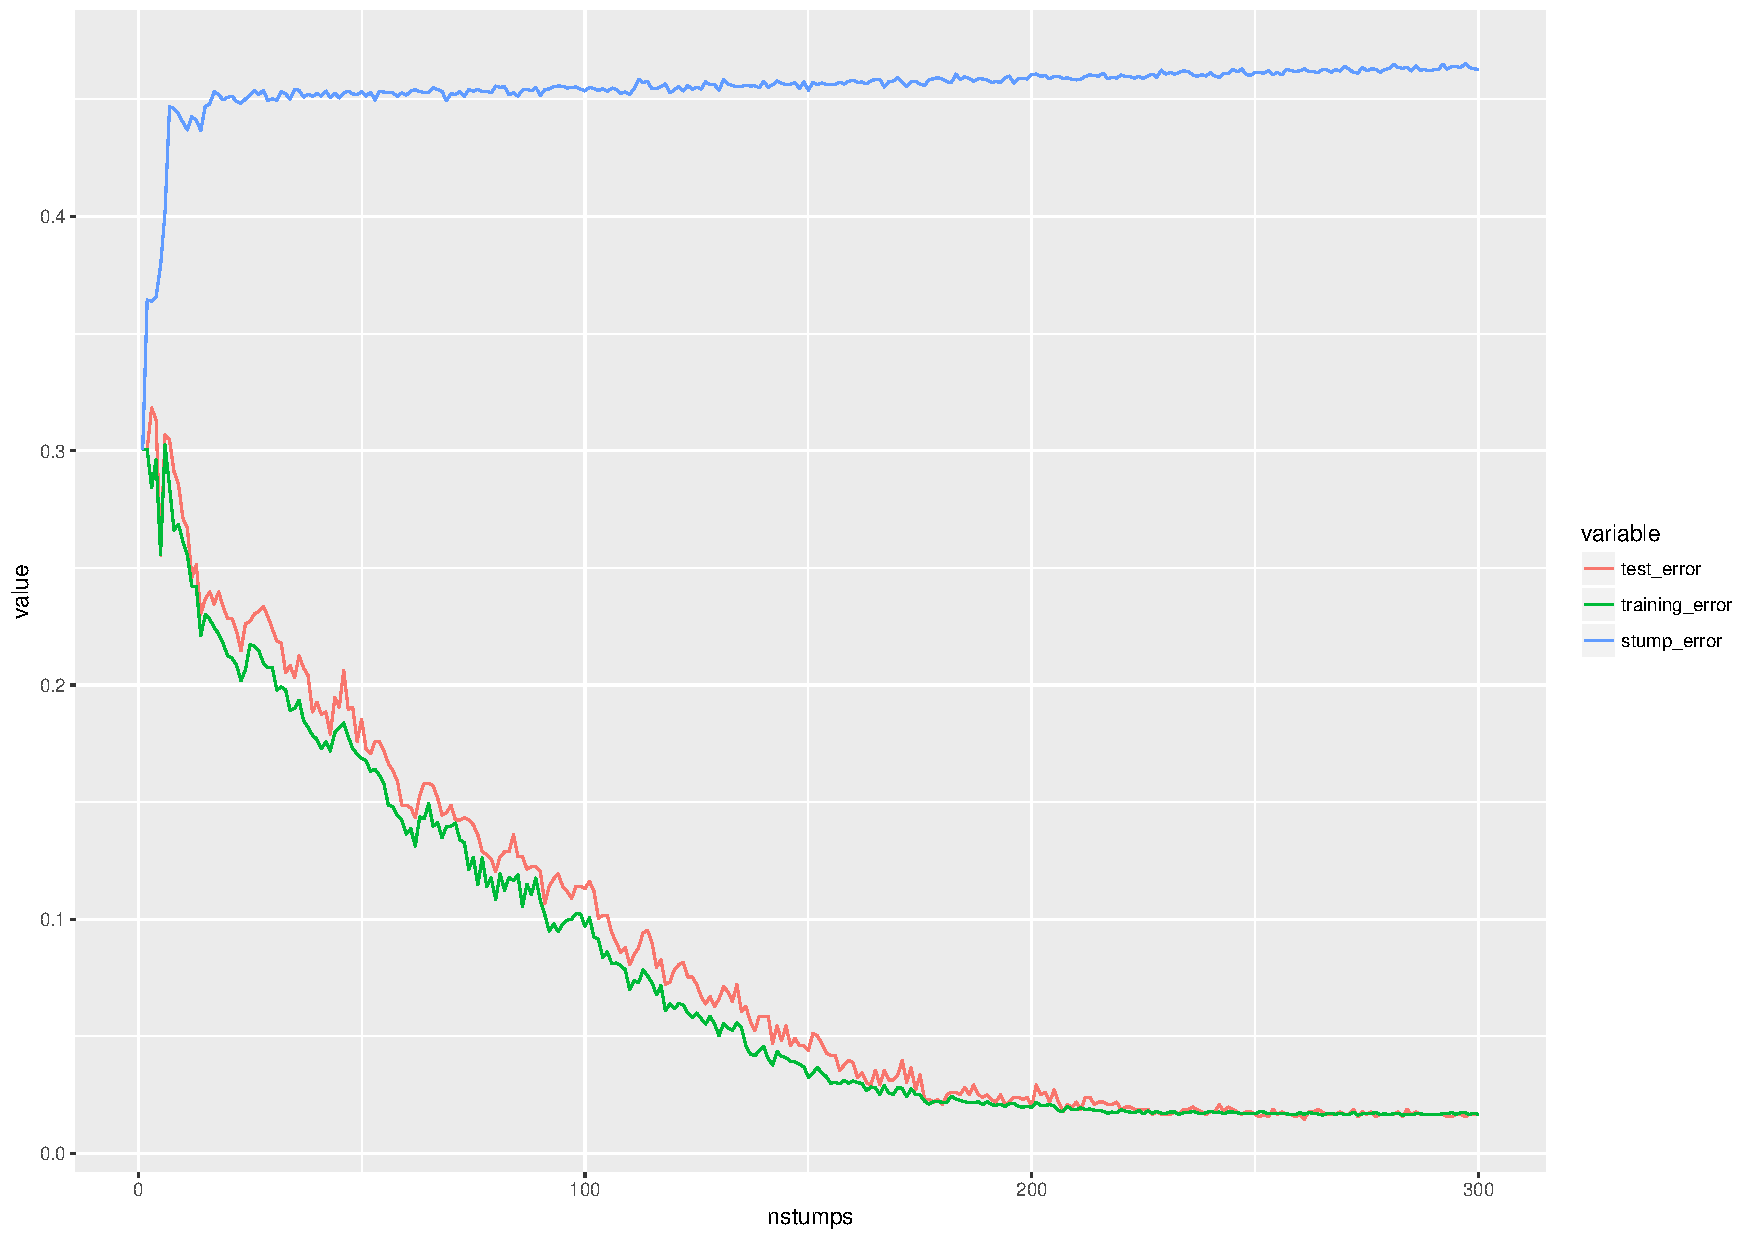
\includegraphics[width=\linewidth]{imgs/accuracy.pdf}
  \caption{Adaboost erros por quantidade de \emph{weak classifiers}}
  \label{fig:adaboostAccuracy}
\end{figure}

\begin{figure}[h]
  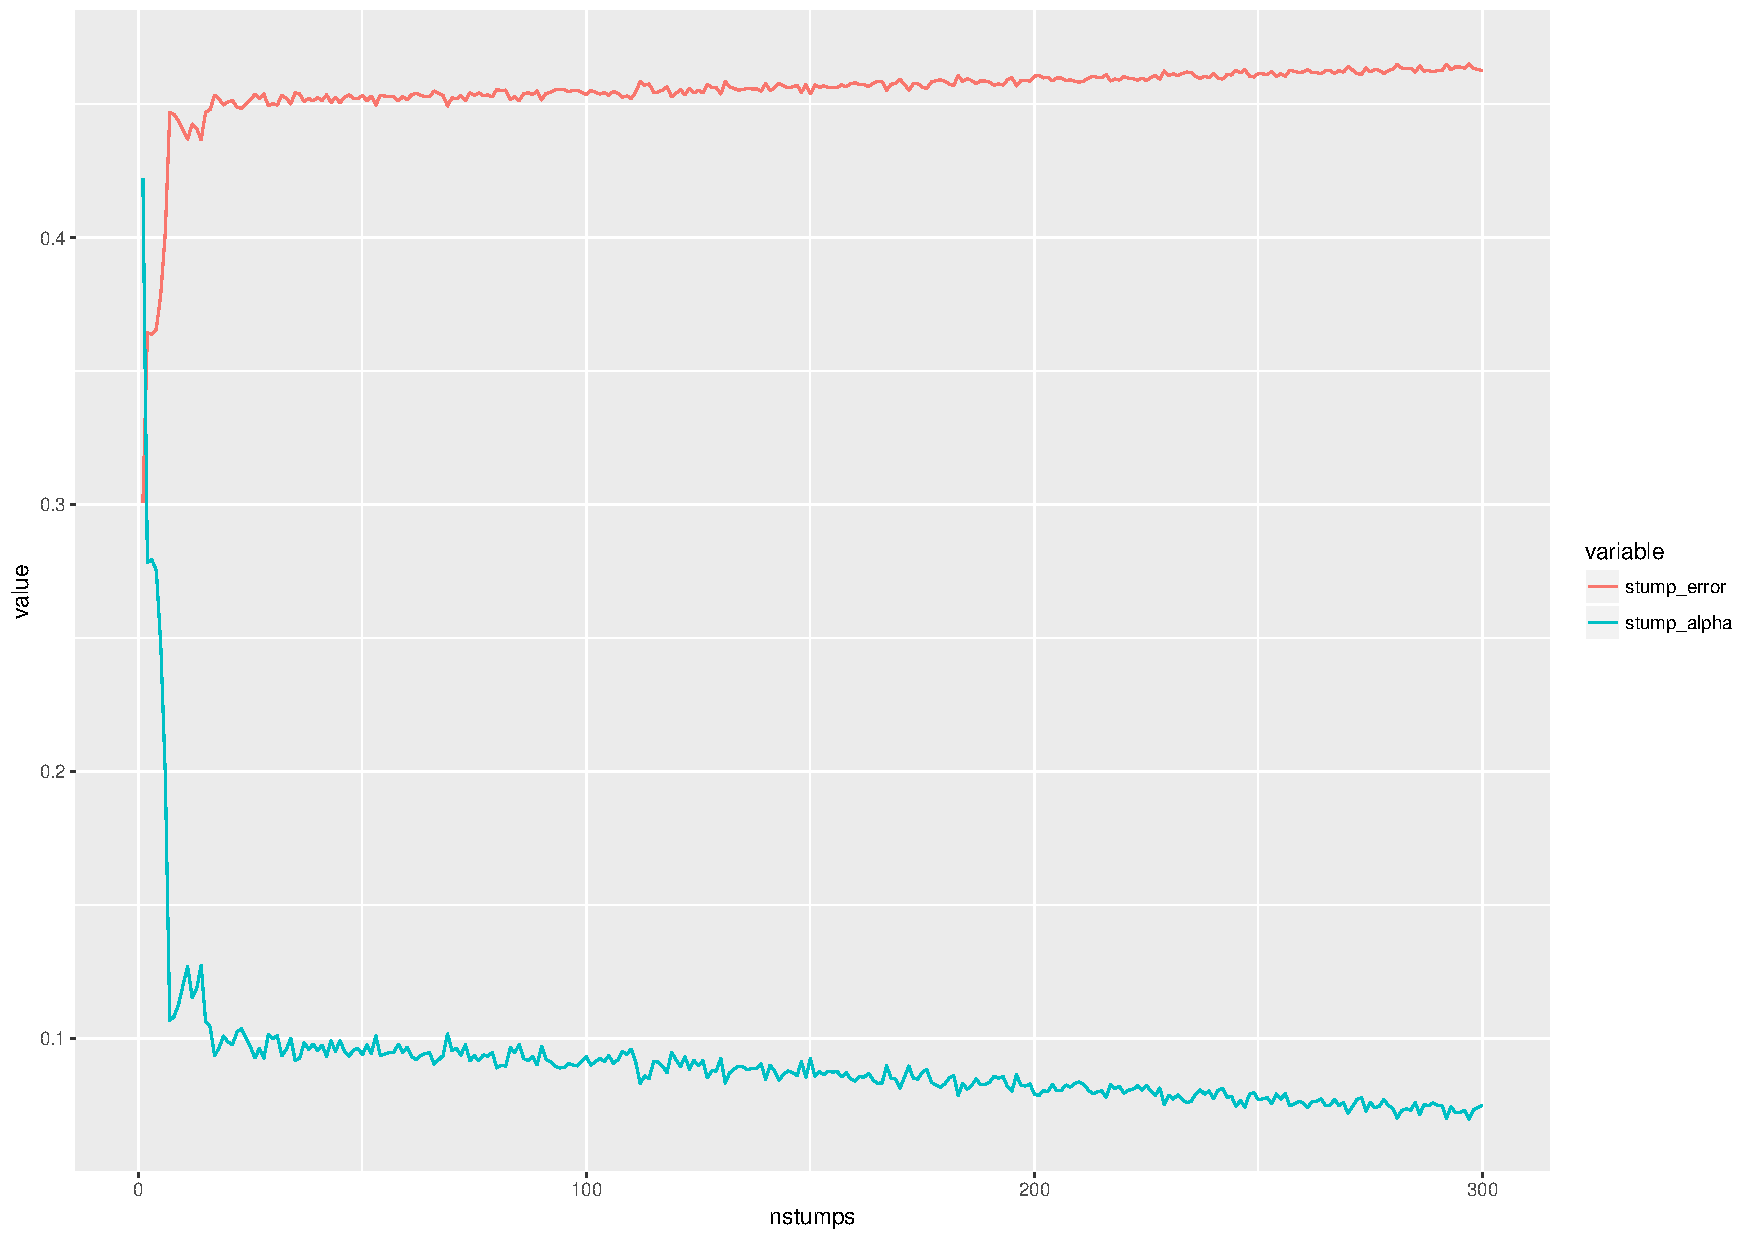
\includegraphics[width=\linewidth]{imgs/alpha_error.pdf}
  \caption{Adaboost \emph{stumps} escolhidos em cada iteração com seus  alphas e errors  associados}
  \label{fig:adaboost_alphas}
\end{figure}
